\section{Istruzioni per l'utilizzo}

\subsection{Primo avvio}
\subsubsection{Autenticazione}
\label{sec:autenticazione}
All'avvio verrà mostrata una schermata che servirà ad autenticarsi, nella quale bisognerà inserire nome utente e password del proprio account \gloman{Zextras Drive} (Figura 4). In caso di successo dell'operazione si avvierà il \gloman{software}, altrimenti verrà visualizzato un messaggio di errore e chiesto di reinserire le credenziali (Figura 5).  \newline
Ai prossimi avvii del software l'account verrà automaticamente caricato, a meno che non venga effettuato il logout (paragrafo x.x.x).
\begin{figure}[H]
    \centering
    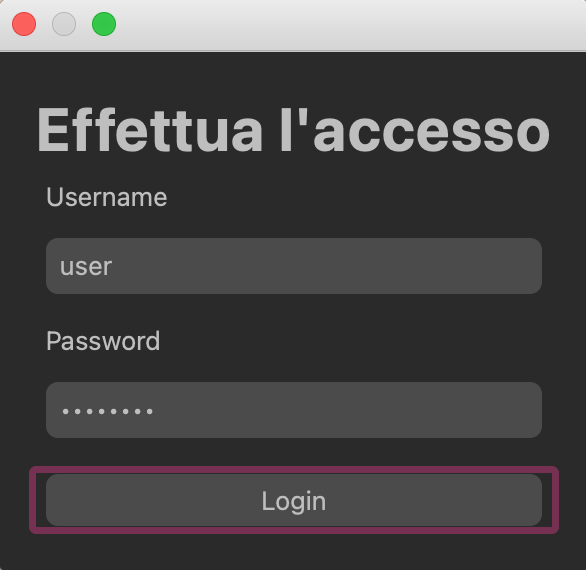
\includegraphics[scale = 0.50]{components/img/login.png}
    \caption{Login}
    \label{fig:Vista del login}
\end{figure}
\begin{figure}[H]
    \centering
    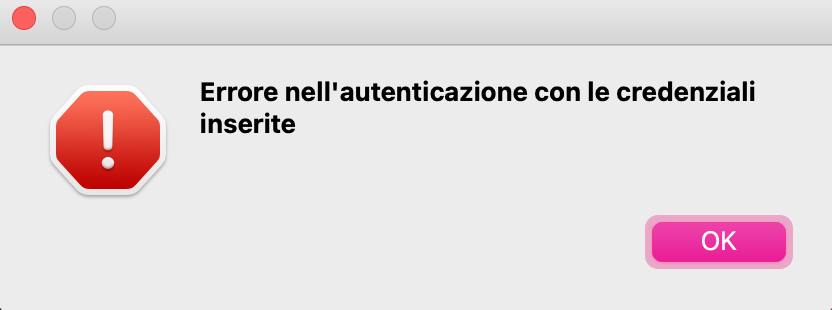
\includegraphics[scale = 0.50]{components/img/err-login.png}
    \caption{Errore di autenticazione}
    \label{fig:Vista del login}
\end{figure}
\subsubsection{Selezione del percorso da sincronizzare}
\label{sec:selezionepath}
Verrà richiesto di scegliere una cartella nella quale verranno sincronizzati tutti i file. Non si deve scegliere la stessa cartella nella quale è contenuto il programma.
\begin{figure}[H]
    \centering
    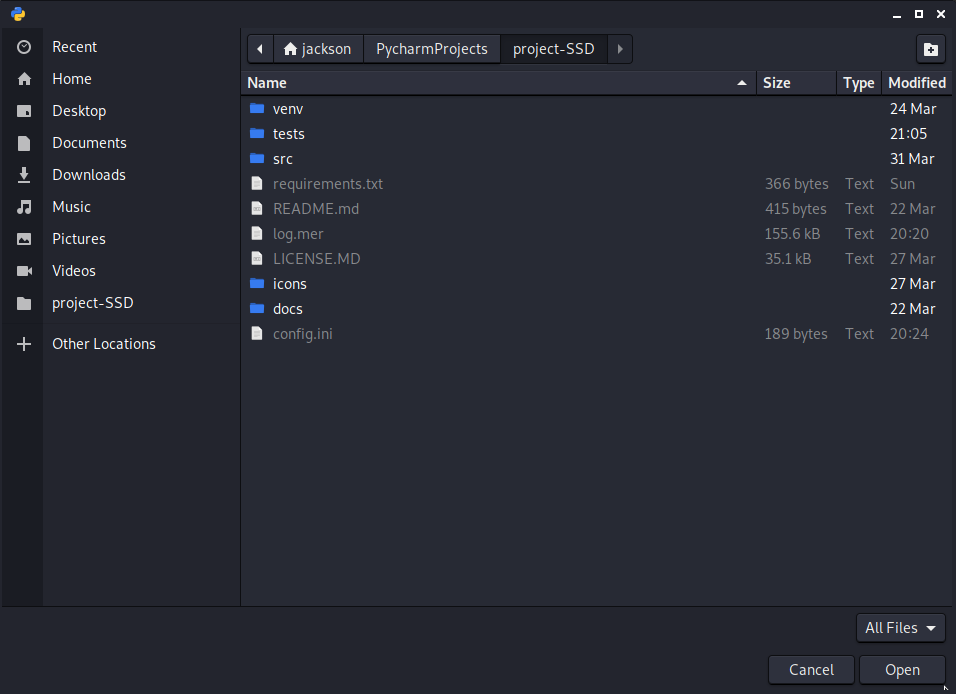
\includegraphics[scale = 0.30]{components/img/selezione-path.png}
    \caption{Selezione del percorso da sincronizzare}
    \label{fig:Selezione del percorso da sincronizzare}
\end{figure}


\subsection{Finestra principale}

\begin{figure}[H]
    \centering
    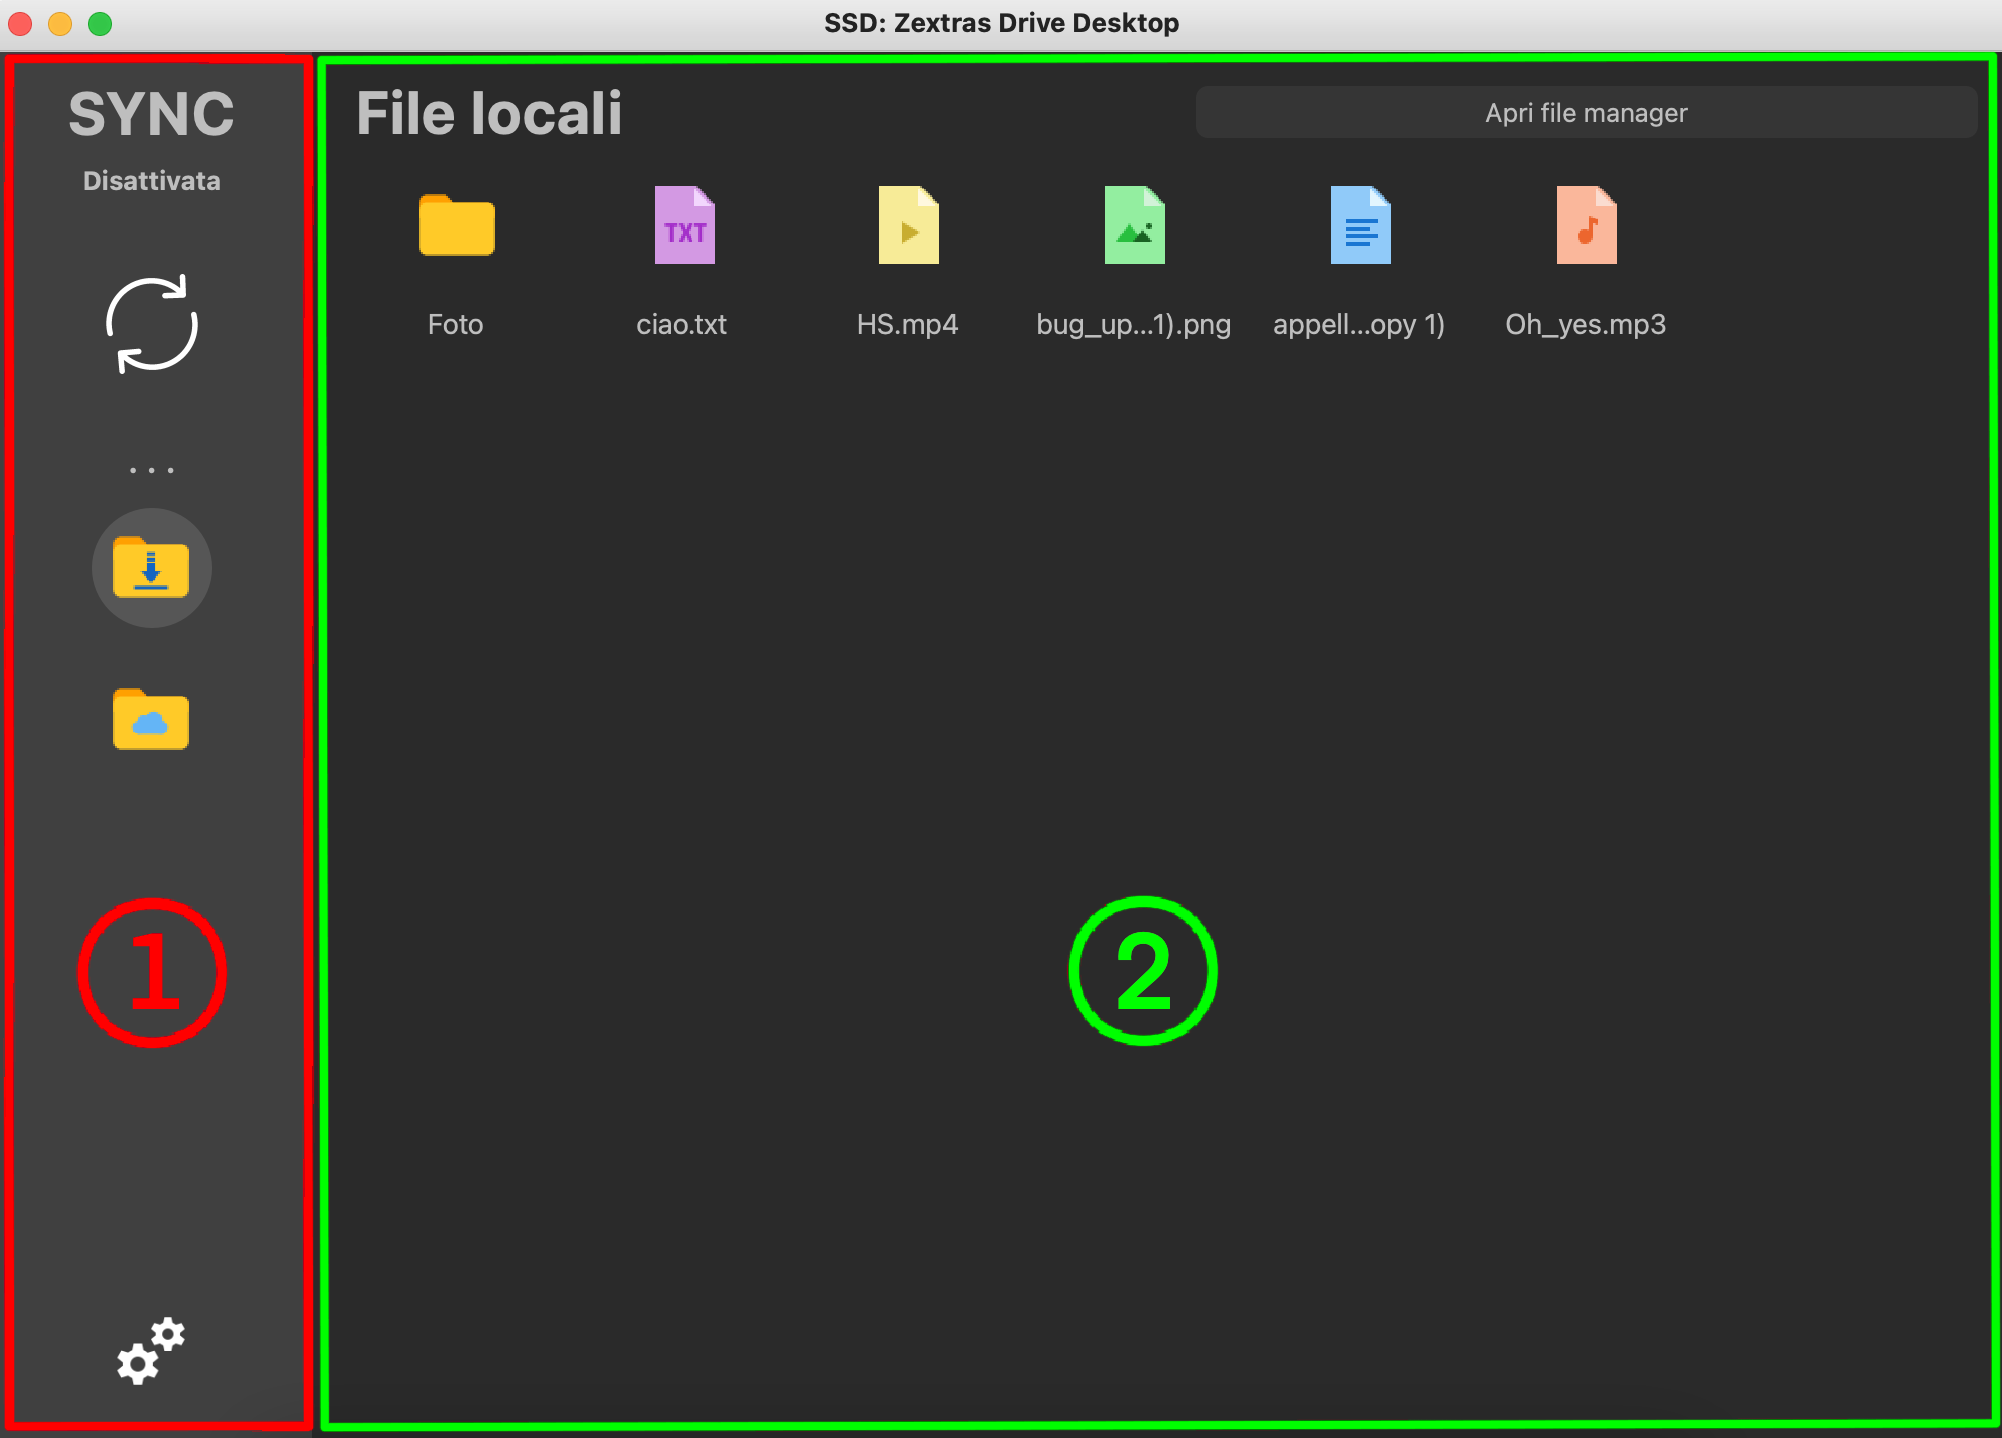
\includegraphics[scale = 0.7]{components/img/Principale.png}
    \caption{Vista schermata principale}
    \label{fig:fileSync}
\end{figure}

Una volta avviato il software si aprirà una finestra, nella quale verranno visualizzati il menù laterale [1] (\S{}\ref{sec:menu}) e la cartella locale [2] (\S{}\ref{sec:fileSincronizzati}).
\subsubsection{Menù laterale}
\label{sec:menu}

Il menù laterale, rappresentato nel punto 1 della Figura 7 è posizionato a sinistra della vista e presenta quattro pulsanti:
\begin{itemize}
\item \textbf{Pulsante di sincronizzazione}: attiva e disattiva la sincronizzazione della cartella locale con il server; \
\end{itemize}

\begin{figure}[H]
\centering
\begin{minipage}[b]{0.45\linewidth}
\centering

\includegraphics[scale=0.5]{components/img/SyncA.png}
\caption{Sincronizzazione attivata}
\label{fig:syncA}
\end{minipage}
\quad
\begin{minipage}[b]{0.45\linewidth}
\centering
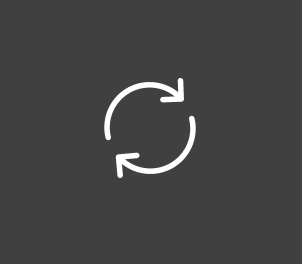
\includegraphics[scale=0.5]{components/img/SyncD.png}
\caption{Sincronizzazione disattivata}
\label{fig:syncD}
\end{minipage}
\end{figure}

\begin{itemize}
\item \textbf{Pulsante file sincronizzati}: mostra la cartella locale sincronizzata (\S{}\ref{sec:fileSincronizzati}); \
\end{itemize}

\begin{figure}[H]
    \centering
    
\includegraphics[scale = 1]{components/img/pulsanteFileS.png}
    \caption{Pulsante file sincronizzati}
    \label{fig:fileSync}
\end{figure}

\begin{itemize}
\item \textbf{Pulsante file remoti}: mostra i file presenti sul server (\S{}\ref{sec:fileRemoti}); \
\end{itemize}

\begin{figure}[H]
    \centering
    
\includegraphics[scale = 1]{components/img/pulsanteFileR.png}
    \caption{Pulsante file remoti}
    \label{fig:fileRem}
\end{figure}

\begin{itemize}
\item \textbf{Pulsante delle impostazioni}: mostra le impostazioni del software (\S{}\ref{sec:impostazioni}). \
\end{itemize}

\begin{figure}[H]
    \centering
    
\includegraphics[scale = 1]{components/img/pulsanteImpostazioni.png}
    \caption{Pulsante impostazioni}
    \label{fig:fileSync}
\end{figure}

\subsubsection{File sincronizzati}
\label{sec:fileSincronizzati}

\begin{figure}[H]
    \centering
    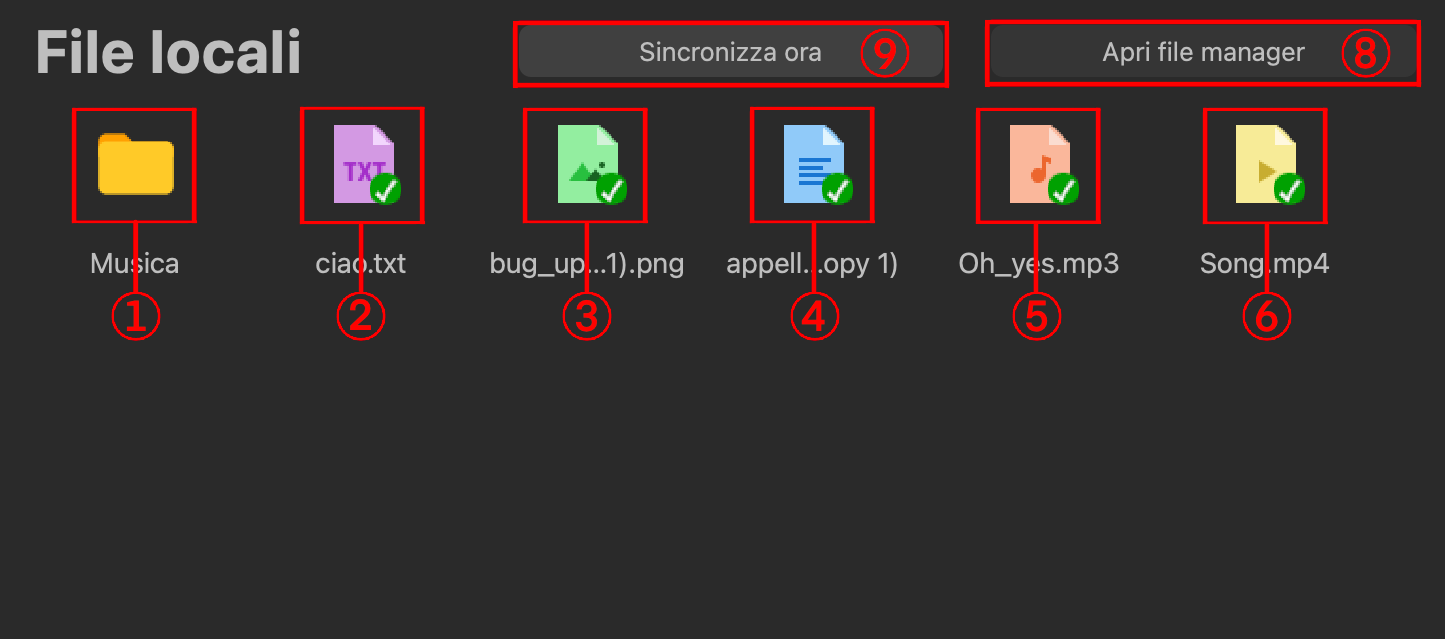
\includegraphics[scale = 0.7]{components/img/fileLocali.png}
    \caption{Vista file locali}
    \label{fig:fileSync}
\end{figure}

La vista si compone di una serie di icone che rappresentanoo i file o le cartelle presenti nella cartella condivisa. Le icone possono rappresentare:

\begin{itemize}
\item \textbf{Cartella [1]};\
\item \textbf{File di testo [2]};\
\item \textbf{File video [3]};\
\item \textbf{File immagine [4]};\
\item \textbf{File generico [5]};\
\item \textbf{File audio [6]}.\
\end{itemize}

In alto a sinistra è presente un pulsante [7] che apre la cartella sincronizzata col file manager del computer.



\subsubsection{File remoti}
\label{sec:fileRemoti}
spiega la vista

\subsubsection{Azioni sui file}

\subsubsection*{Doppio click su un file}

\subsubsection*{Doppio click su una cartella}

\subsubsection*{Inserire file nella cartella locale}
Per far si che un file venga correttamente visualizzato all'interno del software, l'utente può:
\begin{itemize}
\item Creare il file nella cartella; \
\item Spostare nella cartella un file già esistente.
\end{itemize}

\subsubsection*{Sincronizzare file dal server}

\subsubsection*{Refresh del server}

\subsubsection*{Modifica di un file sincronizzato}

\subsubsection*{Cancellazione di un file sincronizzato}

\subsubsection{Impostazioni}
\label{sec:impostazioni}
spiega la vista \newline
modifica path cartella \newline
modifica policy \newline
modifica finestra temporale \newline
modifica spazio di archiviazione (notifica spazio insufficiente) \newline
logout


